\documentclass{sosg-informe}

\graphicspath{{figuras/}{../../mapas-galapagos/capturas/}}

\newcommand{\kmc}{km\textsuperscript{2}}
\newcommand{\mc}{m\textsuperscript{2}}

\title{Base geoespacial y susceptibilidad topográfica\\a inundación (HAND) en los poblados\\de Santa Cruz, San Cristóbal e Isabela}
\titulocorto{Base geoespacial y susceptibilidad HAND}
\numero{2026-01}
\estado{Borrador para discusión}
\titulocita{Base geoespacial y susceptibilidad topográfica a inundación (HAND) en los poblados de Santa Cruz, San Cristóbal e Isabela}
\relacionados{Issues \issue{1}, \issue{2}, \issue{16}, \issue{22}, \issue{23} y \issue{28} · repositorio mayait/sosgalapagos-datos}
\date{4 de noviembre de 2026}

\begin{document}
\maketitle

\begin{abstract}
Tras las lluvias del 30--31 de octubre de 2026 no existía un mapa oficial de amenaza por inundación pluvial para Galápagos: las capas nacionales de la SNGR y del INEC no tienen entidades en las islas. En dos días se integró una base geoespacial común para Santa Cruz, San Cristóbal y el sur de Isabela con la cartografía IGM 1:25\,000, OpenStreetMap, Google Open Buildings, capas de la SNGR, el INEC y el CGREG, y el modelo de superficie Copernicus GLO-30. El servicio WFS del IGM entrega cada elemento repetido por las hojas superpuestas: la deduplicación por geometría reduce 116\,674 elementos a 39\,434, y 2\,800 tramos de quebrada a 909. Sobre el DSM, con las quebradas del IGM quemadas 3~m, se calcularon la red de drenaje D8 con su orden de Strahler, las cuencas completas que drenan a cada poblado (44,2~\kmc{} a Puerto Ayora, 11,5~\kmc{} a Puerto Baquerizo Moreno, 1,4~\kmc{} a Puerto Villamil) y el índice HAND (altura sobre el drenaje más cercano), clasificado en susceptibilidad alta ($\leq 1$~m), media ($\leq 2{,}5$~m) y baja ($\leq 5$~m) a menos de 300~m del cauce. Al cruzarlo con 17\,001 huellas de edificios y 9\,475 viviendas georreferenciadas por la SNGR, quedan en susceptibilidad alta o media unas 5\,550 personas estimadas: el 23\,\% en Santa Cruz, el 8\,\% en San Cristóbal y el 30\,\% en Isabela, donde el terreno plano de Puerto Villamil exagera el índice. El HAND es una medida de posición en el relieve: no tiene caudal ni periodo de retorno, borra los vasos cerrados como La Cascada y no se ha validado con la delimitación de lo inundado. Coincide bien con la quebrada de flujos de lodo del CGREG sobre La Cascada (79\,\% de su área en alguna clase), pero solo cubre el 18\,\% del polígono oficial de riesgo de inundación de Puerto Ayora. Sirve para priorizar, no para delimitar.
\palabrasclave{HAND; susceptibilidad a inundación; modelo digital de superficie; D8; cuencas aportantes; exposición; Galápagos.}
\end{abstract}

\begin{aviso}
Este informe presenta \textbf{modelos propios, no datos oficiales}. La susceptibilidad HAND, las cuencas, los cauces derivados y la costa baja son estimaciones sobre un modelo digital de \emph{superficie} de 30~m; no son un mapa de amenaza ni sirven para normar el uso del suelo. La población es una estimación de la SNGR por vivienda, no un censo. El trabajo lo preparó un equipo asistido por agentes de inteligencia artificial, sin visitas de campo ni revisión profesional externa, y no expresa una posición institucional de la USFQ. Licencias de los datos usados: IGM 1:25\,000 (información pública del Estado ecuatoriano); OpenStreetMap, \textcopyright\ colaboradores de OpenStreetMap, ODbL~1.0 (las bases derivadas conservan la ODbL); Google Open Buildings v3, CC BY 4.0; SNGR/INOCAR, MSP, MINEDUC e INEC, servicios públicos sin licencia declarada; CGREG/FCD, uso con cita (licencia por confirmar). El relieve fue \enquote{produced using Copernicus WorldDEM-30 \textcopyright\ DLR e.V. 2010-2014 and \textcopyright\ Airbus Defence and Space GmbH 2014-2018 provided under COPERNICUS by the European Union and ESA}.
\end{aviso}

% =====================================================================
\section{Introducción}

Santa Cruz, San Cristóbal e Isabela no tienen ríos permanentes. Sus inundaciones pluviales son repentinas: el agua baja por quebradas secas (\enquote{encañadas} o \enquote{cañadas}) y se acumula donde esas quebradas entran en los poblados o donde el terreno forma depresiones. El 30 y el 31 de octubre de 2026 la lluvia inundó el barrio La Cascada, en Puerto Ayora, y desbordó las cañadas Barrio Frío y Divino Niño en Puerto Baquerizo Moreno.

En ese momento no había un mapa oficial de amenaza por inundación pluvial para Galápagos. Las capas nacionales de susceptibilidad de la SNGR y del INEC no tienen entidades en las islas, no hubo activaciones de Copernicus EMS ni del Charter, y la delimitación oficial de las áreas afectadas sigue pendiente (\issue{1}). Para coordinar la respuesta hacía falta, al menos, una base común: quebradas, cuencas, zonas pobladas, vías, servicios y una primera aproximación de dónde se acumularía el agua.

Este informe documenta esa base y el índice con el que se priorizó: HAND (\emph{Height Above Nearest Drainage}; \citealp{renno2008,nobre2011}), la altura de cada punto del terreno sobre el cauce al que drena. Es un índice topográfico, barato y reproducible, que no requiere lluvia ni caudal. Esa misma ventaja es su límite: dice dónde se acumularía primero el agua si una quebrada se desborda, pero no cuánta agua viene ni con qué frecuencia. Los análisis hidrológicos e hidráulicos posteriores (informes 2026-04 a 2026-06) parten de esta base.

% =====================================================================
\section{Área de estudio y datos}

\subsection{Poblados}
El análisis cubre los poblados de las tres islas habitadas con más población:
\begin{itemize}
  \item \textbf{Santa Cruz:} Puerto Ayora, Bellavista y Santa Rosa, más los sectores rurales poblados de la parte alta;
  \item \textbf{San Cristóbal:} Puerto Baquerizo Moreno y El Progreso;
  \item \textbf{Isabela (sur):} Puerto Villamil y la parroquia Tomás de Berlanga (Santo Tomás). No debe confundirse con el sector homónimo de Santa Cruz.
\end{itemize}
Floreana y el resto de Isabela quedan fuera (\issue{15}).

El \textbf{área de interés} une la zona agrícola y la urbana completas (zonificación del Parque Nacional de 2017 y suelo urbano y rural del CGREG), las cuencas completas que drenan a cada poblado (sección~\ref{sec:cuencas}), 500~m alrededor de las zonas pobladas y 300~m alrededor de las vías transitables. Se recorta a la costa con 60~m de margen. Mide 193,5~\kmc{} en Santa Cruz, 108,4~\kmc{} en San Cristóbal y 76,1~\kmc{} en Isabela (figura~\ref{fig:area}). El resto del Parque Nacional se procesa con el mismo método, pero se publica aparte, sin recorte.

\subsection{Fuentes}
La tabla~\ref{tab:fuentes} resume las fuentes, consultadas entre el 31 de octubre y el 1 de noviembre de 2026: IGM \citep{igm25k}, CGREG y FCD \citep{cgreg2017}, SNGR e INOCAR \citep{sngr2026}, INEC \citep{inec2026}, OpenStreetMap \citep{osm2026}, Google Open Buildings \citep{sirko2021} y Copernicus GLO-30 \citep{esa2021}. Cada capa conserva el tipo de dato: \textbf{oficial} (publicado por una institución), \textbf{abierto} (colaborativo o de terceros) o \textbf{modelo} (cálculo propio).

\begin{table}[ht]
  \centering\small
  \caption{Fuentes de la base geoespacial y tipo de dato.}
  \label{tab:fuentes}
  \begin{tabularx}{\linewidth}{>{\raggedright\arraybackslash}p{3.1cm}>{\raggedright\arraybackslash}Xl}
    \toprule
    Fuente & Qué aporta & Tipo \\
    \midrule
    IGM 1:25\,000 & Quebradas, límite urbano, terreno inundable, lagunas, poblados, vías, edificios, puntos acotados, acueductos y puentes (70 capas) & Oficial \\
    CGREG / FCD & Zonificación del Parque (2017), suelo urbano y rural, riesgo de inundación (Puerto Ayora y Puerto Villamil), flujos de lodo por El Niño, encañadas con franja de 20~m, barrios & Oficial \\
    SNGR / INOCAR & Inundación por tsunami, rutas de evacuación, refugios, eventos históricos, 9\,475 viviendas con población estimada & Oficial \\
    MSP, MINEDUC (vía SNGR) & Establecimientos de salud (2023) e instituciones educativas (2021, incompleta) & Oficial \\
    INEC, MGN 2026 & Manzanas y sectores censales & Oficial \\
    OpenStreetMap & Vías, edificios, servicios y uso del suelo (Geofabrik, 31-oct-2026) & Abierto (ODbL) \\
    Google Open Buildings v3 & Huellas de edificios en Santa Cruz e Isabela (no cubre San Cristóbal) & Abierto (CC BY 4.0) \\
    Copernicus GLO-30 & Modelo digital de superficie, 1 segundo de arco (${\approx}\,30{,}9$~m) & Abierto \\
    Derivados propios & Drenaje D8, cuencas, HAND, costa baja, pendientes, exposición & Modelo \\
    \bottomrule
  \end{tabularx}
\end{table}

Las capas oficiales de la SNGR y del MSP traen nombres y teléfonos de responsables de refugios, de fuentes de los eventos y de profesionales de la salud, y la descripción libre de los eventos históricos nombra a personas afectadas. Esos campos se eliminan en el script de integración (\texttt{07\_oficiales.py} y \texttt{08\_exportar.py}); los datos crudos no se publican.

\subsection{El modelo de elevación y su sesgo}\label{sec:dsm}
Copernicus GLO-30 es un modelo digital de \emph{superficie} (DSM) derivado de TanDEM-X: incluye techos y copas de árboles. Su cota se contrastó con los puntos acotados del IGM 1:25\,000 en los estudios de La Cascada y de San Cristóbal (tabla~\ref{tab:dsm}). En el entorno de Puerto Ayora el DSM queda entre 2 y 3~m por debajo del IGM, y más dentro de la zona poblada. En Puerto Baquerizo Moreno el sesgo cambia de signo (${\approx}\,+1{,}5$~m). El error cuadrático medio es de unos 3~m en ambos puertos y de 5~m en El Progreso. Una parte del sesgo probablemente es de referencia vertical (EGM2008 frente al nivel medio del mar del IGM; \issue{12}) y afecta menos a los desniveles locales que a las cotas absolutas. Por eso este informe no usa cotas absolutas del DSM como umbral: el HAND es una diferencia de cotas.

\begin{table}[ht]
  \centering\small
  \caption{Diferencia DSM $-$ punto acotado IGM 1:25\,000 (m). El punto acotado tiene su propio error.}
  \label{tab:dsm}
  \begin{tabular}{lrrrr}
    \toprule
    Ámbito & $n$ & Media & Mediana & RMSE \\
    \midrule
    Santa Cruz, $\leq 5$~km de La Cascada & 468 & $-2{,}1$ & $-2{,}0$ & 2,9 \\
    \quad dentro de la zona poblada & 53 & $-3{,}4$ & $-3{,}4$ & 3,8 \\
    San Cristóbal, isla completa & 2\,087 & $-2{,}9$ & $-2{,}1$ & 6,9 \\
    \quad $\leq 5$~km de Puerto Baquerizo Moreno & 96 & $+1{,}5$ & $+1{,}8$ & 3,0 \\
    \quad $\leq 2$~km de El Progreso & 25 & $+1{,}9$ & $+1{,}5$ & 5,1 \\
    \bottomrule
  \end{tabular}
  \par\vspace{3pt}\raggedright\footnotesize Fuentes: \texttt{geodatos/estudios/la-cascada/datos/resumen.json} y \texttt{geodatos/estudios/san-cristobal/datos/resumen.json} (clave \texttt{validacion\_dsm}).
\end{table}

% =====================================================================
\section{Métodos}

La base se construye con los scripts \texttt{03\_dem.py} a \texttt{08\_exportar.py} de \texttt{geodatos/scripts/}, en ese orden. Todo trabaja en EPSG:4326; las distancias y áreas se convierten con $1^\circ \approx 111\,320$~m, aceptable a menos de $1{,}1^\circ$ del ecuador.

\subsection{Integración y deduplicación}
\begin{itemize}
  \item \textbf{IGM (\texttt{04\_igm\_wfs.py}, \texttt{05\_igm\_limpiar.py}).} Se descargan las 70 capas del WFS. El servicio devuelve cada elemento varias veces porque las hojas 1:25\,000 se superponen. Se calcula el resumen MD5 de la geometría en WKB de cada elemento y se conserva solo la primera aparición; se descartan los elementos fuera de las tres islas y se normaliza el nombre de la isla.
  \item \textbf{Zonas pobladas (\texttt{06\_integrar.py}).} Unión del límite urbano del IGM, de los usos residenciales de OSM y de una \enquote{huella edificada}: cada edificio de OSM e IGM se dilata 35~m, se unen, se erosiona el conjunto 20~m y se conservan las manchas de al menos 1~ha.
  \item \textbf{Edificios (\texttt{07\_oficiales.py}).} Todos los de OSM, más los de Google Open Buildings v3 con confianza $\geq 0{,}70$ que no se solapan con un edificio de OSM.
  \item \textbf{Puntos clave (\texttt{08\_exportar.py}).} Salud, refugios, educación, agua, energía y transporte de MSP, SNGR, MINEDUC, IGM y OSM. Dos puntos de la misma categoría a menos de 40~m se fusionan y se conserva el de fuente oficial.
\end{itemize}

\subsection{Relieve y pendientes}
Para cada isla se recorta el DSM y se marca como mar toda celda con cota $\leq 0{,}5$~m. La pendiente $\beta$ y la orientación $\alpha$ salen de las diferencias centradas, con un paso horizontal $\Delta x = 30{,}87\cos\varphi$~m y $\Delta y = 30{,}87$~m. El relieve sombreado, con el sol a un azimut $A = 315^\circ$ y una elevación $e = 45^\circ$, es
\begin{equation}
  S = \sin e \cos\beta + \cos e \sin\beta \cos(A - \alpha).
\end{equation}
Las pendientes se publican en tres rangos (15--25$^\circ$, 25--35$^\circ$ y $>35^\circ$) como indicio de laderas inestables, sin modelo de movimientos en masa (\issue{32}). Las curvas de nivel salen del DSM suavizado con un filtro gaussiano ($\sigma = 1{,}2$ celdas), cada 10~m.

\subsection{Acondicionamiento hidrológico del DSM}
\textbf{Quemado de cauces.} Para que el flujo siga las quebradas reales y no salte entre valles por errores del DSM, se rasterizan las quebradas del IGM (todas las celdas que tocan) y se baja el terreno 3~m sobre ellas \citep{lindsay2016}:
\begin{equation}
  z_b(i) = z(i) - 3\ \text{m}\cdot \mathbf{1}\bigl[i \in \text{IGM} \cap \text{tierra}\bigr].
\end{equation}
\textbf{Depresiones y zonas planas.} Sobre $z_b$ se rellenan los pozos de una celda y las depresiones cerradas, y se resuelven las zonas planas imponiendo un gradiente artificial hacia su salida, con la biblioteca \texttt{pysheds} \citep{bartos2020}; los algoritmos son del tipo \emph{priority-flood} \citep{barnes2014pf} y de asignación de direcciones en planos \citep{barnes2014flats}. Este paso es necesario para que todo el flujo llegue al mar, pero \textbf{borra los vasos cerrados} (sección~\ref{sec:disc}).

\subsection{Dirección de flujo, acumulación y orden de Strahler}
Cada celda $i$ drena a la vecina $k$ de mayor pendiente descendente entre las ocho \citep[D8;][]{ocallaghan1984}:
\begin{equation}
  d(i) = \arg\max_{k \in N_8(i)} \frac{z_b(i) - z_b(k)}{L_{ik}}, \qquad L_{ik} \in \{\Delta,\ \sqrt{2}\,\Delta\}.
\end{equation}
El área drenada $A_i$ es el área de la propia celda más la de todas las celdas cuyo camino D8 pasa por $i$, con $a_c = (30{,}87\ \text{m})^2$. Se dibuja un cauce donde $A \geq 0{,}1$~\kmc{} y se publica como \enquote{cauce adicional} el tramo con $A \geq 0{,}2$~\kmc{} que no coincide, a 45~m, con una quebrada ya mapeada: son candidatos a revisar en terreno. Cada tramo lleva su orden de Strahler \citep{strahler1957}: los cauces de cabecera tienen orden 1 y, en cada confluencia,
\begin{equation}
  \omega = \begin{cases} \omega_1 + 1 & \text{si } \omega_1 = \omega_2,\\ \max(\omega_1, \omega_2) & \text{si } \omega_1 \neq \omega_2.\end{cases}
\end{equation}

\subsection{Cuencas que drenan a los poblados}\label{sec:cuencas-met}
El script \texttt{07b\_cuencas\_aportantes.py} define dos productos sobre la misma dirección D8:
\begin{itemize}
  \item \textbf{Cuenca completa de cada localidad:} todas las celdas cuyo flujo termina pasando por la localidad, aunque antes cruce otro poblado. La localidad es la unión de sus manzanas del INEC (por código de parroquia) y de su límite urbano del IGM.
  \item \textbf{Subcuencas por punto de entrada:} cada celda se asigna a la primera celda poblada que encuentra aguas abajo. Las entradas que reúnen al menos 0,2~\kmc{} son subcuencas, con el nombre de la quebrada del IGM si está a menos de 150~m; el resto se agrupa como \enquote{escorrentía local} de cada localidad.
\end{itemize}
Seguir el camino D8 celda a celda desde cada una de las $N$ celdas cuesta $O(N^2)$ en el peor caso. Se usa el \textbf{salto de punteros} \citep{hillis1986}. Sea $s^{(0)}(i)$ la celda siguiente aguas abajo (el mar y las celdas terminales apuntan a sí mismas) y $t^{(0)}(i) = i$ si $i$ es poblada y $-1$ si no. En cada iteración
\begin{equation}
  t^{(k+1)}(i) = \begin{cases} t^{(k)}(i) & \text{si } t^{(k)}(i) \neq -1,\\ t^{(k)}\bigl(s^{(k)}(i)\bigr) & \text{si no,}\end{cases}
  \qquad s^{(k+1)}(i) = s^{(k)}\bigl(s^{(k)}(i)\bigr),
\end{equation}
de modo que tras $\lceil \log_2 N \rceil + 1$ iteraciones cada celda conoce su primera celda poblada aguas abajo. La cuenca completa usa la misma idea con una variable lógica (\enquote{llega a la localidad}), propagada con el operador \textsc{o}. El coste total es $O(N \log N)$.

\subsection{Altura sobre el drenaje más cercano (HAND)}
La red de referencia $R$ son las celdas con $A \geq 0{,}5$~\kmc{} más las quebradas del IGM con $A \geq 0{,}05$~\kmc. Para cada celda $i$, sea $c(i)$ la primera celda de $R$ en su camino D8 sobre el DSM quemado. Entonces \citep{renno2008,nobre2011}
\begin{equation}
  \mathrm{HAND}(i) = z(i) - z\bigl(c(i)\bigr),
\end{equation}
con la cota $z$ del DSM \emph{sin quemar}, para no restar los 3~m artificiales. Las clases son:
\begin{equation}
  \text{clase}(i) = \begin{cases}
    \text{alta} & \mathrm{HAND} \leq 1\ \text{m},\\
    \text{media} & 1 < \mathrm{HAND} \leq 2{,}5\ \text{m},\\
    \text{baja} & 2{,}5 < \mathrm{HAND} \leq 5\ \text{m},
  \end{cases}
  \qquad \text{solo si } \operatorname{dist}(i, R) \leq 300\ \text{m}.
\end{equation}
La restricción de distancia evita marcar como susceptibles mesetas planas alejadas de todo cauce. Las clases se filtran con una mediana de $3 \times 3$ celdas y se convierten en polígonos de al menos 2\,500~\mc. Para publicarlas (\texttt{08\_exportar.py}) se recortan al área de interés, se suavizan con un cierre y una apertura morfológicos de 12~m, se descartan las piezas de menos de 1\,500~\mc{} y se publican \textbf{acumuladas}: el polígono de baja contiene al de media y este al de alta.

\subsection{Costa baja}
Se marcan las celdas con cota de 0--3, 3--5 y 5--10~m, con el mismo filtro de mediana y piezas de al menos 3\,000~\mc. Es una referencia para oleaje y marea alta, sin enlace del DSM con el datum del mareógrafo (\issue{75}). Para tsunami se usa la capa oficial del INOCAR.

\subsection{Exposición}
Cada edificio recibe la clase HAND máxima de los polígonos que \emph{toca} (no la de su centroide), si está en la franja de 20~m de quebradas del CGREG, si toca la zona de tsunami del INOCAR y si su punto representativo está en la costa de 0--3~m. Las viviendas de la SNGR reciben las mismas etiquetas y se suma su población estimada (\texttt{pob\_x\_casa}). La población por manzana del INEC es la suma de esas viviendas dentro de cada manzana, no una cifra censal (\issue{22}).

% =====================================================================
\section{Resultados}

\subsection{Base integrada}
La deduplicación del IGM redujo las 70 capas de 116\,674 a 39\,434 elementos en las tres islas (tabla~\ref{tab:igm}). El factor se acerca a 3 en las capas con muchas hojas, como las quebradas (2\,800 a 909) y los puntos acotados (96\,292 a 29\,231), y es casi 1 en las capas puntuales pequeñas. El paquete publicado tiene 25 capas; las principales se cuentan en la tabla~\ref{tab:capas}.

\begin{table}[ht]
  \centering\small
  \caption{Deduplicación del WFS del IGM 1:25\,000 (elementos de las tres islas).}
  \label{tab:igm}
  \begin{tabular}{lrrrrr}
    \toprule
    Capa & Original & Depurada & Santa Cruz & San Cristóbal & Isabela \\
    \midrule
    Quebradas (\texttt{rio}) & 2\,800 & 909 & 138 & 282 & 489 \\
    Puntos acotados & 96\,292 & 29\,231 & 8\,498 & 2\,125 & 18\,608 \\
    Vías & 3\,932 & 1\,966 & 952 & 739 & 275 \\
    Edificios (puntos) & 2\,819 & 2\,707 & 1\,577 & 847 & 283 \\
    Terreno inundable & 64 & 32 & 24 & 2 & 6 \\
    Límite urbano & 18 & 5 & 3 & 1 & 1 \\
    \midrule
    Las 70 capas & 116\,674 & 39\,434 & & & \\
    \bottomrule
  \end{tabular}
\end{table}

\begin{table}[ht]
  \centering\small
  \caption{Capas principales del paquete publicado (\texttt{geodatos/export/galapagos/}, recortado al área de interés).}
  \label{tab:capas}
  \begin{tabularx}{\linewidth}{>{\raggedright\arraybackslash}Xrl}
    \toprule
    Capa & Elementos & Tipo \\
    \midrule
    Susceptibilidad a inundación por quebradas (HAND, clases acumuladas) & 2\,558 & Modelo \\
    Cauces adicionales detectados en el relieve (D8, no mapeados) & 1\,324 & Modelo \\
    Quebradas y cauces mapeados (IGM y OSM) & 286 & Oficial y abierto \\
    Cuencas completas que drenan a cada poblado & 7 & Modelo \\
    Subcuencas por punto de entrada & 82 & Modelo \\
    Costa baja (0--3, 3--5 y 5--10~m) & 184 & Modelo \\
    Inundación por tsunami (INOCAR) & 449 & Oficial \\
    Zonas inundables y de riesgo oficiales (IGM y CGREG) & 54 & Oficial \\
    Edificios expuestos (alguna etiqueta) & 6\,598 & Abierto + modelo \\
    Población estimada por manzana & 820 & Oficial (estimación) \\
    Puntos clave (salud, refugios, servicios) & 692 & Oficial y abierto \\
    \bottomrule
  \end{tabularx}
\end{table}

\subsection{Drenaje y cuencas}\label{sec:cuencas}
La figura~\ref{fig:area} muestra el área de interés, las quebradas del IGM, los cauces derivados no mapeados y las cuencas completas de cada localidad (tabla~\ref{tab:cuencas}). Tres resultados destacan:
\begin{itemize}
  \item \textbf{Puerto Ayora recibe el agua de 44,2~\kmc}, que incluyen los 15,6~\kmc{} de Bellavista: lo que llueve en la parte alta de Santa Cruz pasa por dos poblados antes de llegar al mar.
  \item \textbf{La cartografía oficial no tiene la mayor parte de los cauces.} Se publicaron 1\,324 tramos derivados del DSM que no coinciden con ninguna quebrada mapeada: 755 en Santa Cruz, 243 en San Cristóbal y 326 en Isabela. El orden de Strahler de esos tramos llega a 6 en Santa Cruz y a 5 en San Cristóbal e Isabela. San Cristóbal es la isla mejor cartografiada: el IGM tiene allí 282 quebradas.
  \item \textbf{Santa Rosa y El Progreso} reciben muy poca área (0,3 y 0,1~\kmc) porque están sobre lomas. Que el resultado sea real, y no un efecto del DSM, está por confirmar en terreno.
\end{itemize}

\begin{table}[ht]
  \centering\small
  \caption{Cuencas completas que drenan a cada localidad (modelo D8 sobre el DSM con las quebradas del IGM quemadas). El área aguas arriba excluye la propia localidad.}
  \label{tab:cuencas}
  \begin{tabular}{llrr}
    \toprule
    Isla & Localidad & Cuenca completa (\kmc) & Aguas arriba (\kmc) \\
    \midrule
    Santa Cruz & Puerto Ayora & 47,2 & 44,2 \\
    Santa Cruz & Bellavista & 17,2 & 15,6 \\
    Santa Cruz & Santa Rosa & 0,8 & 0,3 \\
    San Cristóbal & Puerto Baquerizo Moreno & 14,5 & 11,5 \\
    San Cristóbal & El Progreso & 0,5 & 0,1 \\
    Isabela & Tomás de Berlanga (Santo Tomás) & 11,6 & 10,8 \\
    Isabela & Puerto Villamil & 3,0 & 1,4 \\
    \bottomrule
  \end{tabular}
\end{table}

\begin{figure}[t]
  \centering
  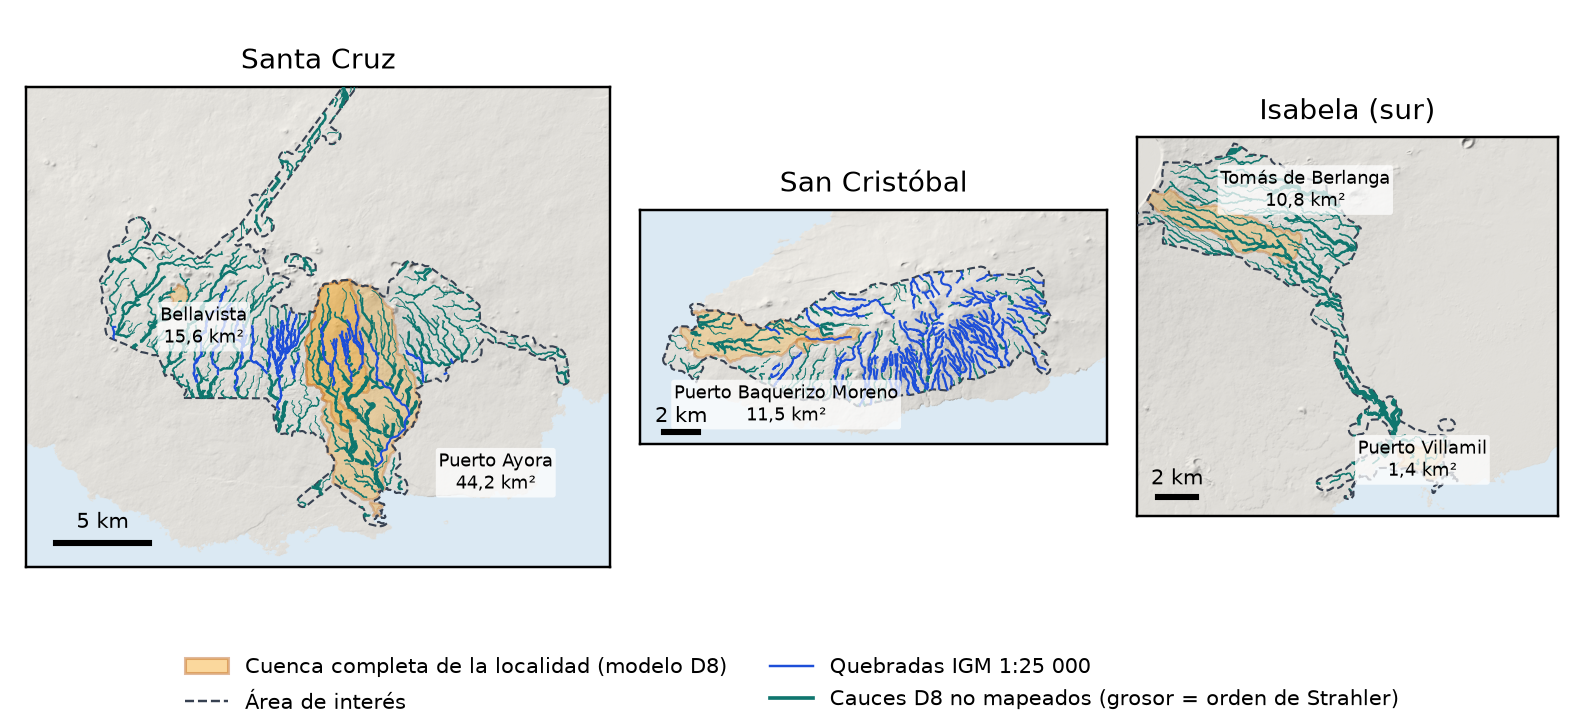
\includegraphics[width=\linewidth]{area_estudio.png}
  \caption{Área de interés, quebradas del IGM 1:25\,000, cauces derivados del DSM que no coinciden con una quebrada mapeada (grosor según el orden de Strahler) y cuencas completas que drenan a cada localidad, con su área aguas arriba. Fondo: relieve sombreado del DSM Copernicus GLO-30. Cuencas y cauces son modelo.}
  \label{fig:area}
\end{figure}

\subsection{Susceptibilidad HAND}
La capa publicada tiene 2\,558 polígonos (tabla~\ref{tab:capas}): 1\,316 en Santa Cruz, 784 en San Cristóbal y 458 en Isabela. La figura~\ref{fig:hand} la muestra en los tres puertos junto a las capas oficiales del CGREG. En Puerto Ayora la clase alta sigue las quebradas que bajan del escarpe y la franja de la quebrada de La Cascada; en Puerto Baquerizo Moreno, casi solo la encañada Galápagos (Barrio Frío). En Puerto Villamil, en cambio, el índice cubre buena parte del poblado: el terreno es tan plano que muchas celdas quedan a menos de 1~m de algún cauce derivado.

Para describir la coincidencia con las capas oficiales se midió la fracción del área de cada polígono del CGREG cubierta por las clases acumuladas (tabla~\ref{tab:solape}). \textbf{No es una validación}: los polígonos del CGREG no delimitan un evento ni dicen con qué criterio se trazaron.
\begin{itemize}
  \item El polígono de \textbf{flujos de lodo por El Niño} sobre la quebrada de La Cascada coincide bien: el 79\,\% de su área está en alguna clase y el 38\,\% en la alta.
  \item El polígono de \textbf{riesgo de inundación de Puerto Ayora} coincide poco: solo el 4\,\% de su área está en la clase alta y el 18\,\% en alguna clase. Cubre sobre todo la franja costera baja del centro (Pelican Bay, Las Ninfas), lejos de los cauces de referencia. Allí el problema parece de acumulación en terreno bajo, que el HAND no representa; está por comprobar si la capa de costa baja lo describe mejor.
  \item En San Cristóbal, los polígonos de flujos de lodo siguen la Galápagos; el 61\,\% de su área está en alguna clase.
\end{itemize}
La documentación del repositorio afirma que la clase alta \enquote{coincide} con el polígono de riesgo de Puerto Ayora; la tabla~\ref{tab:solape} matiza esa afirmación: la coincidencia es parcial y se limita a los bordes del polígono que tocan cauces.

\begin{table}[ht]
  \centering\small
  \caption{Fracción del área de los polígonos oficiales del CGREG cubierta por las clases HAND publicadas (acumuladas). Indicador descriptivo calculado por \texttt{figuras.py} de este informe; no es una validación.}
  \label{tab:solape}
  \begin{tabular}{lrccc}
    \toprule
    Polígono del CGREG & Área (ha) & Alta & Media o más & Alguna clase \\
    \midrule
    Flujos de lodo por El Niño, Santa Cruz (La Cascada) & 18,3 & 38\,\% & 68\,\% & 79\,\% \\
    Flujos de lodo por El Niño, San Cristóbal & 47,5 & 7\,\% & 36\,\% & 61\,\% \\
    Riesgo de inundación, Puerto Ayora & 87,3 & 4\,\% & 15\,\% & 18\,\% \\
    Riesgo de inundación, Puerto Villamil & 361,3 & 11\,\% & 16\,\% & 18\,\% \\
    \bottomrule
  \end{tabular}
\end{table}

\begin{figure}[t]
  \centering
  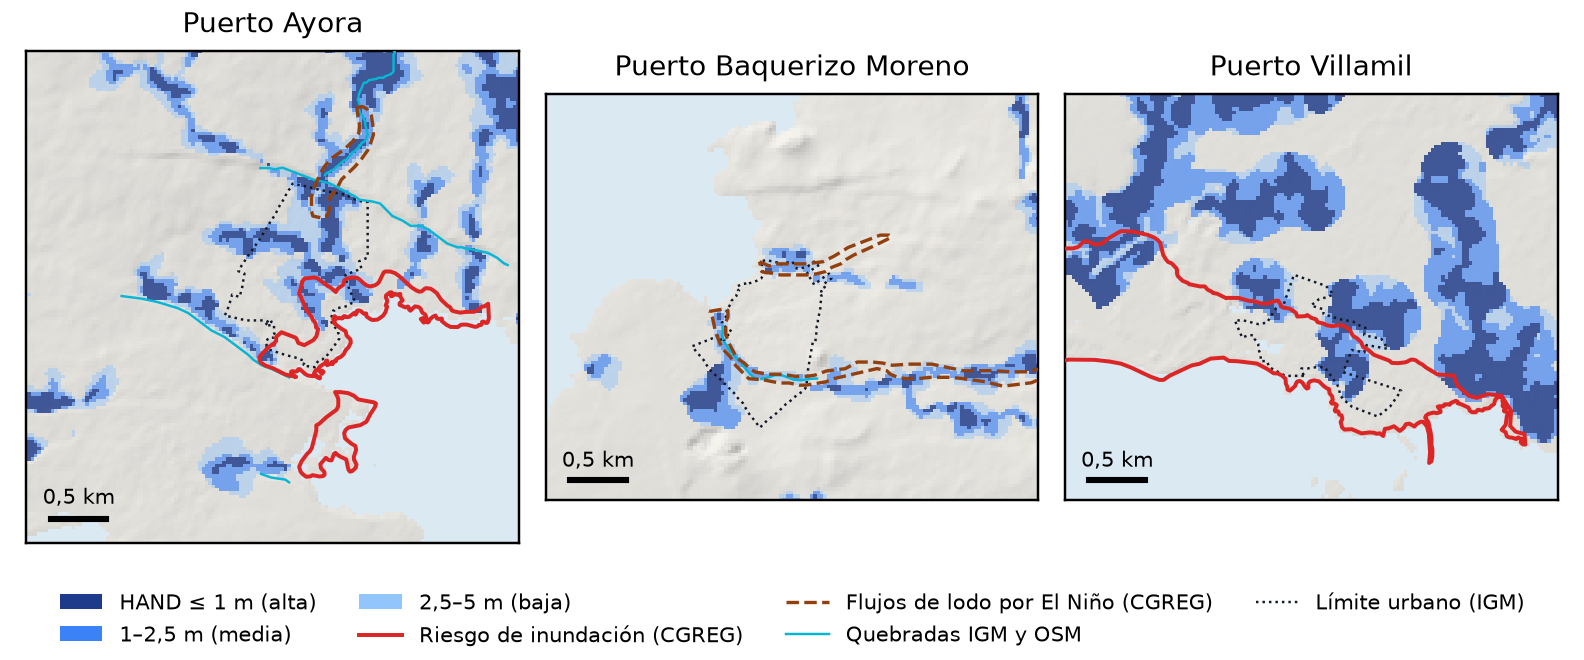
\includegraphics[width=\linewidth]{hand_poblados.png}
  \caption{Clases HAND en Puerto Ayora, Puerto Baquerizo Moreno y Puerto Villamil (ráster de 30~m antes del suavizado de publicación), con los polígonos oficiales de riesgo de inundación y de flujos de lodo por El Niño del CGREG, las quebradas mapeadas y el límite urbano del IGM. El HAND es modelo; los polígonos del CGREG son oficiales.}
  \label{fig:hand}
\end{figure}

\subsection{Exposición}
La tabla~\ref{tab:expo} y la figura~\ref{fig:expo} resumen \texttt{resumen\_exposicion.json}. En las tres islas hay 17\,001 edificios y 28\,060 personas estimadas. En susceptibilidad alta o media quedan 2\,960 edificios y unas 5\,550 personas (20\,\%):
\begin{itemize}
  \item \textbf{Santa Cruz:} 2\,014 edificios (19\,\%) y 3\,965 personas (23\,\%). Es la isla con más personas expuestas en cifras absolutas.
  \item \textbf{San Cristóbal:} 409 edificios (9\,\%) y 657 personas (8\,\%). En cambio, es la única isla con exposición significativa en la franja de 20~m de quebradas del CGREG: 172 edificios y 228 personas, porque esa franja del CGREG cubre las encañadas de Puerto Baquerizo Moreno y no existe en Puerto Ayora.
  \item \textbf{Isabela:} 537 edificios (26\,\%) y 928 personas (30\,\%). La proporción más alta se debe en buena parte a la sobrestimación del HAND en el terreno plano de Puerto Villamil, que además tiene más población en zona de tsunami (1\,064 personas) que en susceptibilidad HAND.
\end{itemize}
Las cifras de edificios cuentan cada edificio que \emph{toca} un polígono; con el centroide serían algo menores. La población viene de 9\,475 viviendas de la SNGR con población estimada; sus totales por isla coinciden en orden de magnitud con el censo de 2022, pero no son cifras censales.

\begin{table}[ht]
  \centering\small
  \caption{Exposición estimada por isla (edificios OSM + Open Buildings; población estimada por la SNGR por vivienda). \enquote{Alta}, \enquote{media} y \enquote{baja}: clase HAND máxima que toca el edificio.}
  \label{tab:expo}
  \begin{tabular}{lrrr}
    \toprule
    & Santa Cruz & San Cristóbal & Isabela \\
    \midrule
    Edificios & 10\,350 & 4\,579 & 2\,072 \\
    \quad en susceptibilidad alta & 926 & 77 & 381 \\
    \quad en susceptibilidad media & 1\,088 & 332 & 156 \\
    \quad en susceptibilidad baja & 1\,472 & 337 & 102 \\
    \quad en la franja de quebradas de 20~m (CGREG) & 31 & 172 & 0 \\
    \quad en zona de tsunami (INOCAR) & 1\,081 & 190 & 685 \\
    \quad en costa de 0--3~m (modelo) & 162 & 3 & 80 \\
    \addlinespace
    Población estimada & 16\,880 & 8\,094 & 3\,086 \\
    \quad en susceptibilidad alta o media & 3\,965 & 657 & 928 \\
    \quad en la franja de quebradas de 20~m & 4 & 228 & 0 \\
    \quad en zona de tsunami & 917 & 207 & 1\,064 \\
    \bottomrule
  \end{tabular}
\end{table}

\begin{figure}[t]
  \centering
  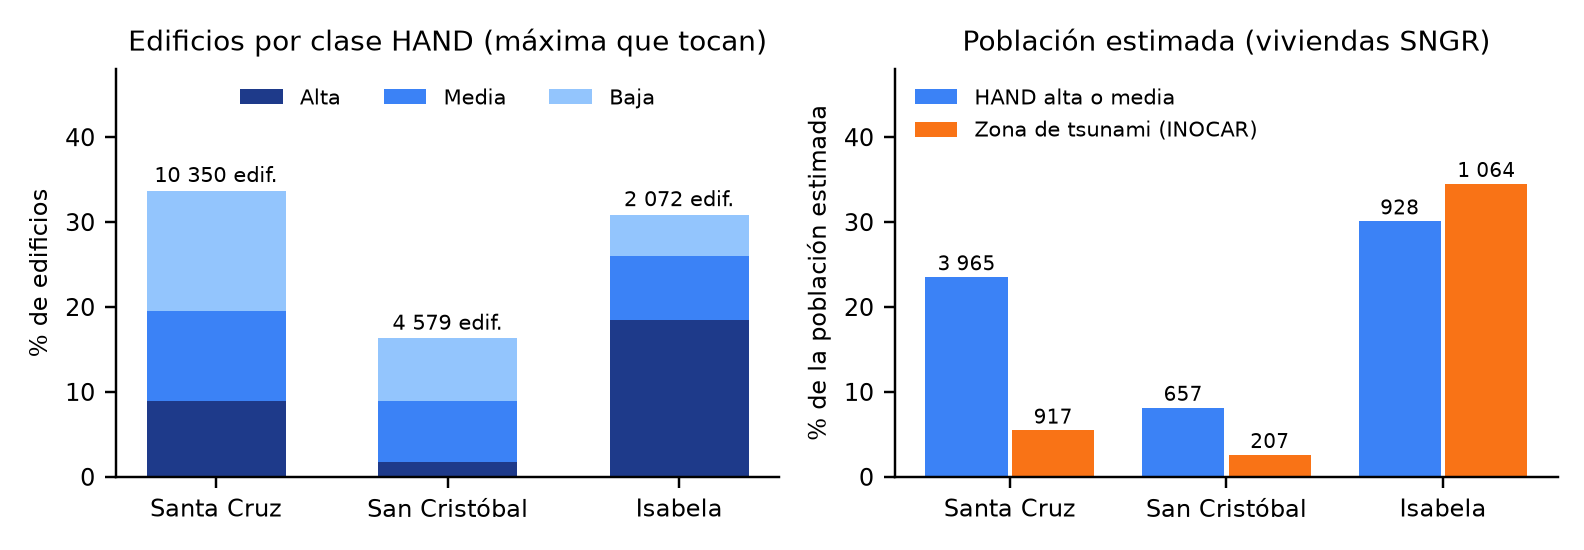
\includegraphics[width=\linewidth]{exposicion.png}
  \caption{Izquierda: porcentaje de edificios de cada isla según la clase HAND máxima que tocan. Derecha: porcentaje de la población estimada (viviendas SNGR) en susceptibilidad alta o media y en zona de tsunami del INOCAR, con las cifras absolutas sobre las barras.}
  \label{fig:expo}
\end{figure}

\subsection{Producto publicado}
Las capas se publican con su manifiesto (\texttt{capas.json}) en el visor de mapas del proyecto y en el entregable \texttt{mapas-galapagos/}, con descargas en GeoJSON y Shapefile (figura~\ref{fig:visor}). Cada capa de modelo lleva en su leyenda que sirve para priorizar y no es una delimitación oficial.

\begin{figure}[t]
  \centering
  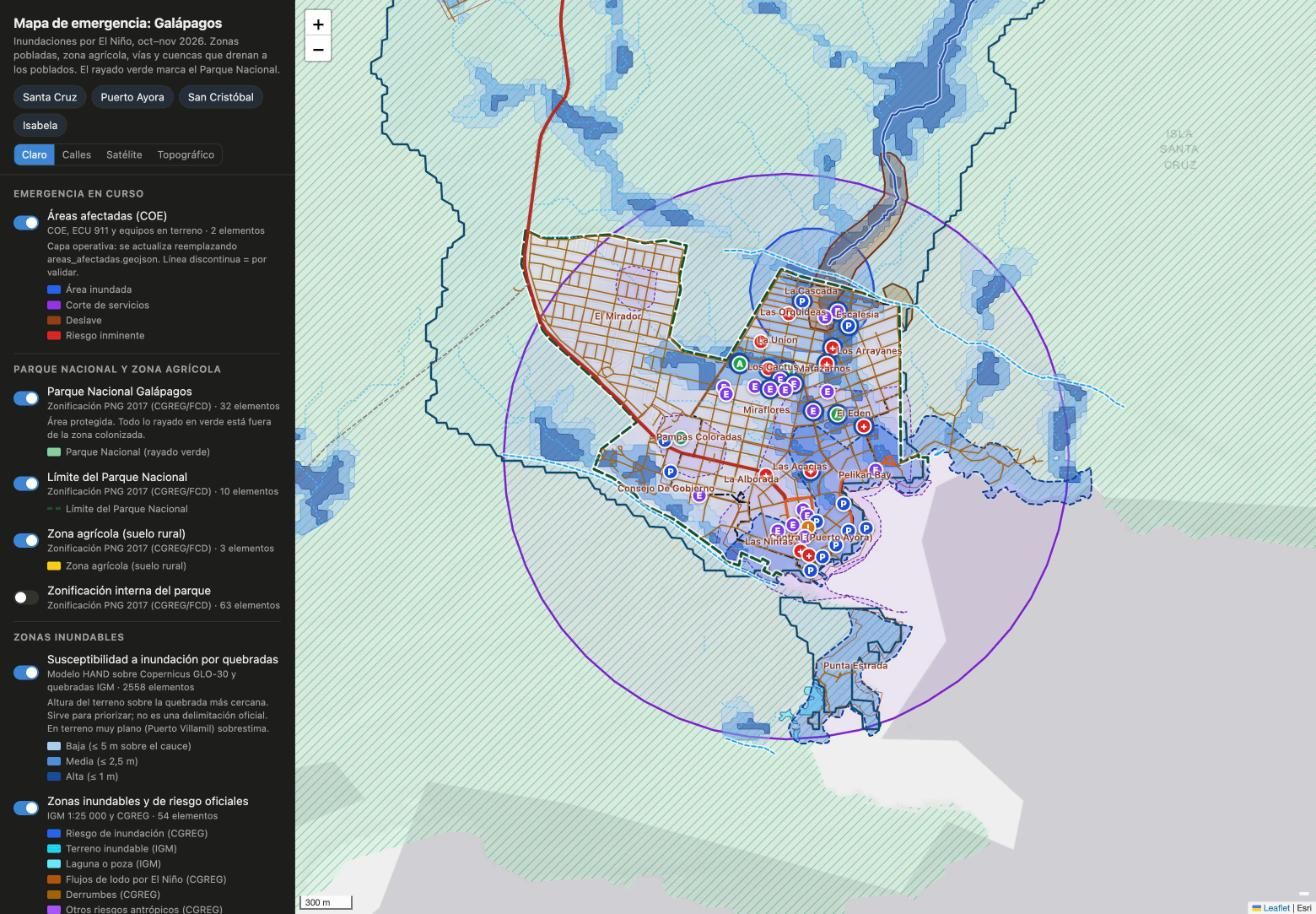
\includegraphics[width=0.9\linewidth]{01-puerto-ayora.jpg}
  \caption{Visor de mapas de la emergencia en Puerto Ayora: susceptibilidad HAND (azules), zonas inundables oficiales, cuencas, quebradas, Parque Nacional (rayado) y puntos clave. Captura de \texttt{mapas-galapagos/capturas/}.}
  \label{fig:visor}
\end{figure}

% =====================================================================
\section{Discusión y limitaciones}\label{sec:disc}

HAND normaliza el terreno respecto a la red de drenaje y, en cuencas con cauces bien definidos, su contorno aproxima la extensión de las inundaciones \citep{nobre2016}. En Galápagos el índice cumple su función de priorizar: resalta las quebradas que bajan del escarpe hacia Puerto Ayora y la encañada Galápagos en Puerto Baquerizo Moreno, y casi toda la quebrada de flujos de lodo del CGREG sobre La Cascada. Pero tiene límites que deben decirse cada vez que se muestra el mapa:
\begin{itemize}
  \item \textbf{El DSM es de superficie.} Techos y árboles elevan la cota en la ciudad y en el bosque de la parte alta, y su sesgo frente al IGM es de $-2$ a $-3$~m en Santa Cruz y de signo contrario en Puerto Baquerizo Moreno (tabla~\ref{tab:dsm}). Un edificio de dos plantas junto al cauce puede quedar \enquote{alto} sin serlo. Las cotas absolutas no sirven como umbral.
  \item \textbf{30~m de resolución.} El DSM no ve cauces estrechos, muros, alcantarillas ni pasos bajo vías (\issue{5}). En la ciudad el agua sigue las calles, que el modelo no representa.
  \item \textbf{Sobrestimación en terreno plano.} En Puerto Villamil casi todo queda a menos de 2,5~m de algún cauce derivado. Allí el índice dice poco más que \enquote{el terreno es bajo y plano}, y la restricción de 300~m no basta para corregirlo. Sus cifras de exposición son las menos fiables.
  \item \textbf{Vasos cerrados.} El relleno de depresiones, imprescindible para trazar el flujo, \enquote{borra} las cuencas endorreicas. La Cascada es un vaso cerrado con 42,3~\kmc{} drenando hacia él y fue el barrio más afectado el 30-oct; el HAND solo marca la quebrada que llega al barrio, no el vaso. Esos lugares se analizan aparte (informes 2026-04 y 2026-05).
  \item \textbf{Sin caudal ni periodo de retorno.} Es posición topográfica, no una simulación. Dos celdas con el mismo HAND pueden recibir caudales muy distintos según el área que drena hacia ellas. Pasar de susceptibilidad a amenaza requiere un modelo hidrológico e hidráulico por periodo de retorno (\issue{25}, \issue{26}, \issue{28}).
  \item \textbf{Umbrales convencionales.} Las clases de 1, 2,5 y 5~m y el área de cauce de 0,5~\kmc{} no se calibraron. Con marcas de agua podrían ajustarse (\issue{2}, \issue{23}).
  \item \textbf{Validación solo cualitativa.} No existe la delimitación oficial de lo inundado el 30--31 de octubre (\issue{1}) ni marcas de agua levantadas con GNSS (\issue{2}). El único contraste posible es con polígonos del CGREG de origen y criterio desconocidos, y da resultados mixtos (tabla~\ref{tab:solape}).
  \item \textbf{Exposición.} Open Buildings no cubre San Cristóbal, donde los edificios dependen de OSM. La población es la estimada por la SNGR por vivienda; la del censo de 2022 por manzana no está publicada (\issue{8}, \issue{22}). El conteo por contacto con el polígono tiende a sobrestimar frente al conteo por centroide.
\end{itemize}

Hay además una observación sobre el código: el comentario de \texttt{03\_dem.py} dice que la susceptibilidad se restringe a \enquote{400~m del cauce}, pero el cálculo usa 300~m, que es el valor documentado. Las cifras de este informe corresponden a 300~m.

% =====================================================================
\section{Conclusiones y trabajo futuro}
\begin{enumerate}
  \item En dos días se integró una base geoespacial común y reproducible para tres islas, con el tipo de dato (oficial, abierto o modelo) marcado en cada capa y sin datos personales publicados.
  \item La deduplicación del WFS del IGM es imprescindible: sin ella, cada quebrada aparecería unas tres veces.
  \item La mayor parte de los cauces que llegan a los poblados no está en la cartografía oficial. Puerto Ayora drena 44,2~\kmc, incluida toda Bellavista.
  \item Unas 5\,550 personas estimadas (el 20\,\%) viven en susceptibilidad HAND alta o media, con la cifra de Isabela inflada por el terreno plano de Puerto Villamil.
  \item El HAND coincide bien con la quebrada de flujos de lodo sobre La Cascada, pero poco con el polígono de riesgo de inundación de Puerto Ayora, que corresponde sobre todo a la costa baja. Sirve para priorizar inspecciones, no para delimitar zonas ni para normar.
\end{enumerate}

Para pasar de susceptibilidad a amenaza hacen falta:
\begin{itemize}
  \item la delimitación oficial de las áreas inundadas y marcas de agua con GNSS (\issue{1}, \issue{2});
  \item un modelo del terreno de $\leq 1$~m de dron o LiDAR en los poblados (\issue{16}), con el que recalcular el HAND con el mismo script y validarlo (\issue{23});
  \item el datum vertical del IGM frente a EGM2008 (\issue{12}) y el inventario de alcantarillas y pasos bajo vías (\issue{5}, \issue{33});
  \item la población del censo por manzana (\issue{8}, \issue{22}) y huellas de edificios completas en San Cristóbal (\issue{18});
  \item modelos lluvia--caudal e hidráulicos por periodo de retorno, como base de un mapa de amenaza que pueda proponerse como oficial (\issue{25}, \issue{26}, \issue{28}).
\end{itemize}

\section*{Disponibilidad de datos y código}
{\small Todo el procesamiento es reproducible desde el repositorio público \emph{mayait/sosgalapagos-datos}, carpeta \texttt{geodatos/} (Python 3.12; dependencias en \texttt{geodatos/requirements.txt}; \texttt{pysheds} 0.5 con \texttt{numpy} $< 2.4$):
\begin{itemize}
  \item \texttt{scripts/03\_dem.py}: relieve, pendientes, curvas, quemado, D8, Strahler, cuencas al mar, HAND y costa baja;
  \item \texttt{scripts/04\_igm\_wfs.py} y \texttt{05\_igm\_limpiar.py}: descarga y deduplicación del IGM (\texttt{capas/igm/\_resumen.json});
  \item \texttt{scripts/06\_integrar.py}: zonas pobladas, hidrografía y primera exposición;
  \item \texttt{scripts/07\_oficiales.py}: capas oficiales depuradas, edificios combinados y \texttt{resumen\_exposicion.json};
  \item \texttt{scripts/07b\_cuencas\_aportantes.py}: cuencas completas y subcuencas por salto de punteros;
  \item \texttt{scripts/08\_exportar.py}: recorte al área de interés, suavizado y paquete \texttt{export/galapagos/}.
\end{itemize}
Los datos crudos (\texttt{geodatos/descargas/}) no se publican porque contienen datos personales; se regeneran con los scripts 01--07. Las figuras~\ref{fig:area}, \ref{fig:hand} y \ref{fig:expo} y la tabla~\ref{tab:solape} se generan con \texttt{informes/2026-01-base-hand/figuras.py}. La explicación divulgativa del método está en \texttt{docs/modelo-hand.md}. Este informe se compila con \texttt{informes/compilar.sh 2026-01-base-hand}.\par}

\bibliographystyle{sosg}
\bibliography{referencias,bib-2026-01}

\end{document}
